\subsection{Using MDL Heuristic in Climate Data Clustering}
\label{ssc:climate}

We added the linear manifold clustering MDL heuristic into the LMCLUS algorithm,
and tested clustering performance on climate datasets.

Our dataset comprised of subset of the CRU 3.22 dataset of monthly global
surface temperature averages, and Global Precipitation Climatology Centre
(GPCC) dataset of monthly precipitation averages, for a 30 year period form
1951 to 1980.
Original datasets have the same $1^\circ \times 1^\circ$ resolution.
Both datasets are 12 dimensional, so the combined dataset has 24 dimensions.
For each of group of 12 fields, a unit length normalization was performed,
by subtracting the minimum value from every point and divided it by the field
maximum minus the minimum value. Normalization makes the scale of the disparate
temperature and precipitation fields similar.

The K{\"o}ppen-Geiger (KG) climate classification system is a widely used scheme
developed by geographers to classify climate types correlated  with observed
land ecosystems \cite{Koppen:1936dg}. It is based on observed limits of these
ecosystems relative to seasonal or annual precipitation and temperature.
A recent updated version identifies 34 climate classes \cite{Kottek:2006wd}.
The system is not perfect, so variations are often proposed.  However, on
the hypothesis that ecosystem types are an expression of the climate,
the KG system offers a good benchmark for a clustering analysis.
\IfClass{IEEEtran}{}
{
Because the KG system relies on at least seasonal (4) and annual values for
temperature and precipitation, it may be considered 10-dimensional clustering or
classification. Thus, we expect $k$-means clustering to yield less accurate
classes, and  linear manifold clustering might identify more refined classes.
(It is beyond the scope of this paper whether LMC offers improved climate
classification over that derived by geographers' expert knowledge, but this will
be treated in a later paper).
}

We perform clustering of the above climate dataset using following algorithms:
$k$-Means \cite{Jain:1999mf}, ORCLUS \cite{Aggarwal:2000AY}, original
LMCLUS \cite{Haralick:2007rt} and LMCLUS modified with the MDL heuristic.

The $k$-Means clustering assumes that the data is modeled as a mixture of
spherically shaped distributions. In this model, the cluster ideal is a point,
the cluster center, which is its mean, and the observations are isotropically
perturbed around the mean. Because the number of clusters must be set a priori
for $k$-Means, with the climate data clustering, we set this number to 34 to
match the number of Koeppen-Geiger classes. Similarly to $k$-Means, ORCLUS
requires an exact number of clusters as a parameter, but the resulting clusters
are linear manifolds of the dimension specified by one of the parameters.
We set ORLCUS parameters such that the algorithm would generate 34 1D linear
manifold clusters.

Linear Manifold Clustering (LMCLUS) does not have to specify an exact number of
clusters in advance, but there are multiple parameters that affect performance
of the algorithm. We set only a small group of them, the rest of the parameters
were set to their default values. The effect of the parameters
\IfClass{IEEEtran}{}{
\footnote{Appendix section~\ref{sec:lmclus-params} contains LMCLUS parameters,
their description and default values.}
}
on the clustering performance is described in the original paper \cite{Haralick:2007rt}.
In our experiments, the following LMCLUS parameters were set:
\emph{best\_bound} to 0.4, \emph{sampling\_factor} to 0.1,
\emph{number\_of\_clusters} to 34, \emph{min\_cluster\_size} to 150.

We updated LMCLUS with the MDL heuristic that allowed a goodness evaluation
of the prospective manifold cluster before committing to the partitioning of
this clusters from the rest of the dataset. We calculated a compression ratio
as a ratio between ``raw'' cluster encoding, as a total number of bits required
to encode each point of the cluster with a constant precision, and
the cluster MDL encoding. If the compression ratio is larger than a user
specified threshold, the cluster is accepted.

In order to compare the goodness of produced clusterings, we calculated
the total MDL value of the resulting clustering for each algorithm as a sum of
cluster MDL values. We performed the total MDL calculation with various
quantization error values to understand how precision affects it.

We calculated value of the approximate MDL Eq.~\eqref{eq:mdl-lmc-final} for
the climate data clusterings, generated by various algorithms, with
the quantization error $\varepsilon$ in
the interval $\left[0.001, 0.002, \dots, 0.01 \right]$.
Because the quantization error is a parameter for the MDL heuristic,
we calculated separate clusterings for every $\varepsilon$ value in
the specified interval. Moreover, the quantization error affects the calculation
of the compression ratio, thus the compression ratio parameter was
selected different for every clustering calculation as well.
We used the clustering, generated by the original LMCLUS algorithm, for
calculation of an average $\mu$ and a standard deviation $\sigma$ of
a cluster compression ratio at every $\varepsilon$ value.
These statistics were used to bootstrap the compression ratio parameter
for the MDL heuristic. The compression ratio set to $\mu-\sigma/2$ value for
corresponding $\varepsilon$ value.

Figure~\ref{fig:mdl-error} shows that when MDL heuristics is enabled, it
produced clusterings that are slightly different from the clustering generated
by original method. We suspected that Eq.~\eqref{eq:mdl-lmc-final} does not
appropriately reflect the MDL value of the the distribution of the data points
in each of the clusters.

\begin{figure}[ht]
\centering
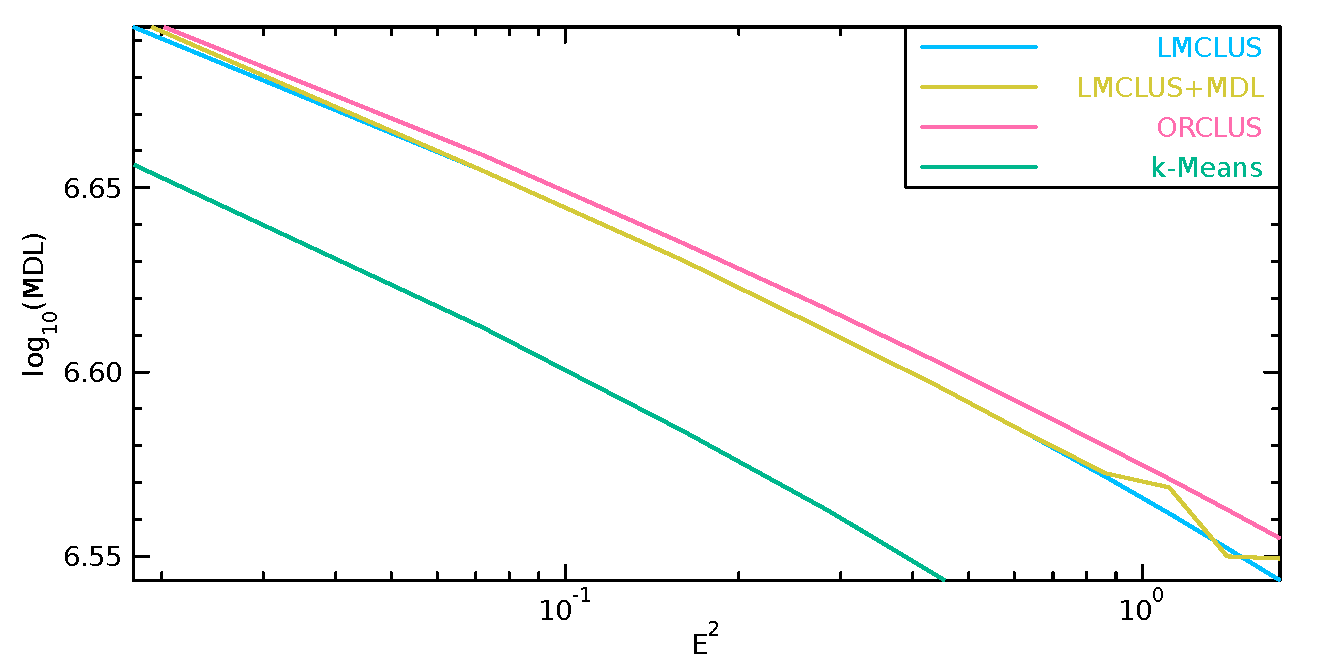
\includegraphics[scale=\IfClass{IEEEtran}{0.3}{0.5}]{img/toterrs2-mdl-oq.pdf}
\IfClass{IEEEtran}{\vspace*{-10pt}}{}
\caption{Clustering optimal quantization MDL value \eqref{eq:mdl-lmc-final} and its squared quantization error for $\varepsilon$ in interval $\left[0.001, 0.002, \dots, 0.01 \right]$ and various algorithms.}
\label{fig:mdl-error}
\end{figure}

When we switched to the ``population'' MDL Eq.~\eqref{eq:mdl-lmc-final-pop}
calculations in our MDL heuristics, with the parameters accordingly recalculated
for this algorithm, performance of the clustering algorithm considerably improved.

It became clear that the effect of the MDL heuristics of resulting clustering,
see Figure~\ref{fig:mdl-error-pop}, are aligned with results from the synthetic
simulation from section \ref{ssc:zero-dim-mdl}. Increasing the precision of
the linear manifold MDL calculation results in better goodness-of-fit qualities
of clusters and allows the filtering of subpar cluster candidates during
the LMCLUS stochastic search, which improves the final clustering.

\begin{figure}[ht]
\centering
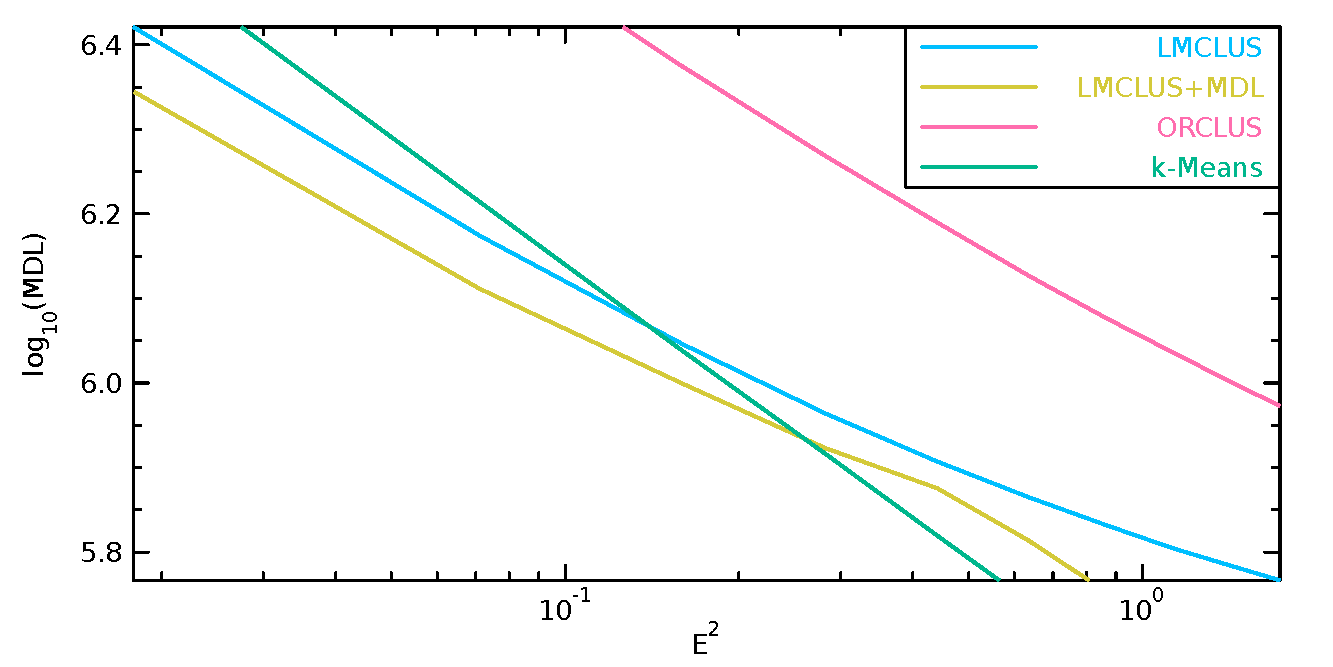
\includegraphics[scale=\IfClass{IEEEtran}{0.3}{0.5}]{img/toterrs2-mdl-si.pdf}
\IfClass{IEEEtran}{\vspace*{-10pt}}{}
\caption{Clustering population MDL value \eqref{eq:mdl-lmc-final-pop} and its squared quantization error for $\varepsilon$ in interval $\left[0.001, 0.002, \dots, 0.01 \right]$ and various algorithms.}
\label{fig:mdl-error-pop}
\end{figure}


\IfClass{IEEEtran}{}{
Figure~\ref{fig:cl-climate} show resulted clusterings plotted on the world map,
where patches of the land are associated with particular clusters.
%
\begin{figure}[ht]
\captionsetup{justification=centering,margin={0cm,-2cm}}
\vspace*{-20pt}
\hspace*{-15pt}
\subfigure[LMCLUS]{
    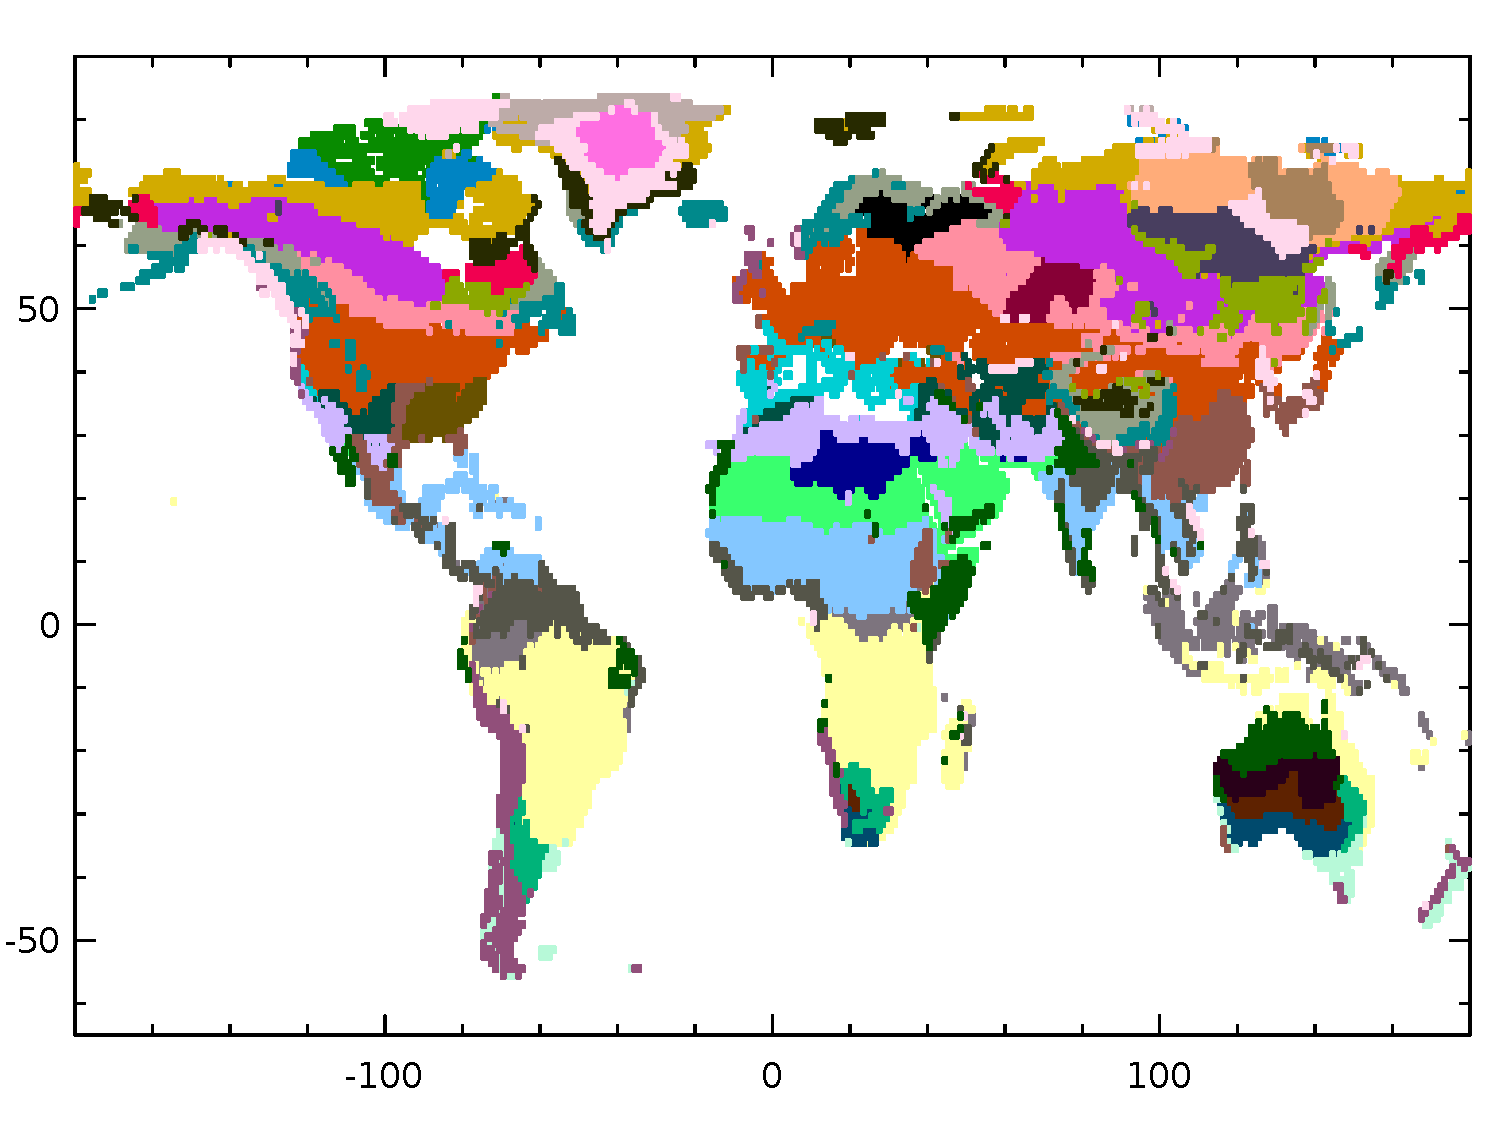
\includegraphics[width=3.5in, height=2.5in]{img/icpr-cl-lmclus.pdf}
    \label{fig:cl-lmclus}}
\hspace*{-15pt}
\subfigure[LMCLUS-MDL]{
    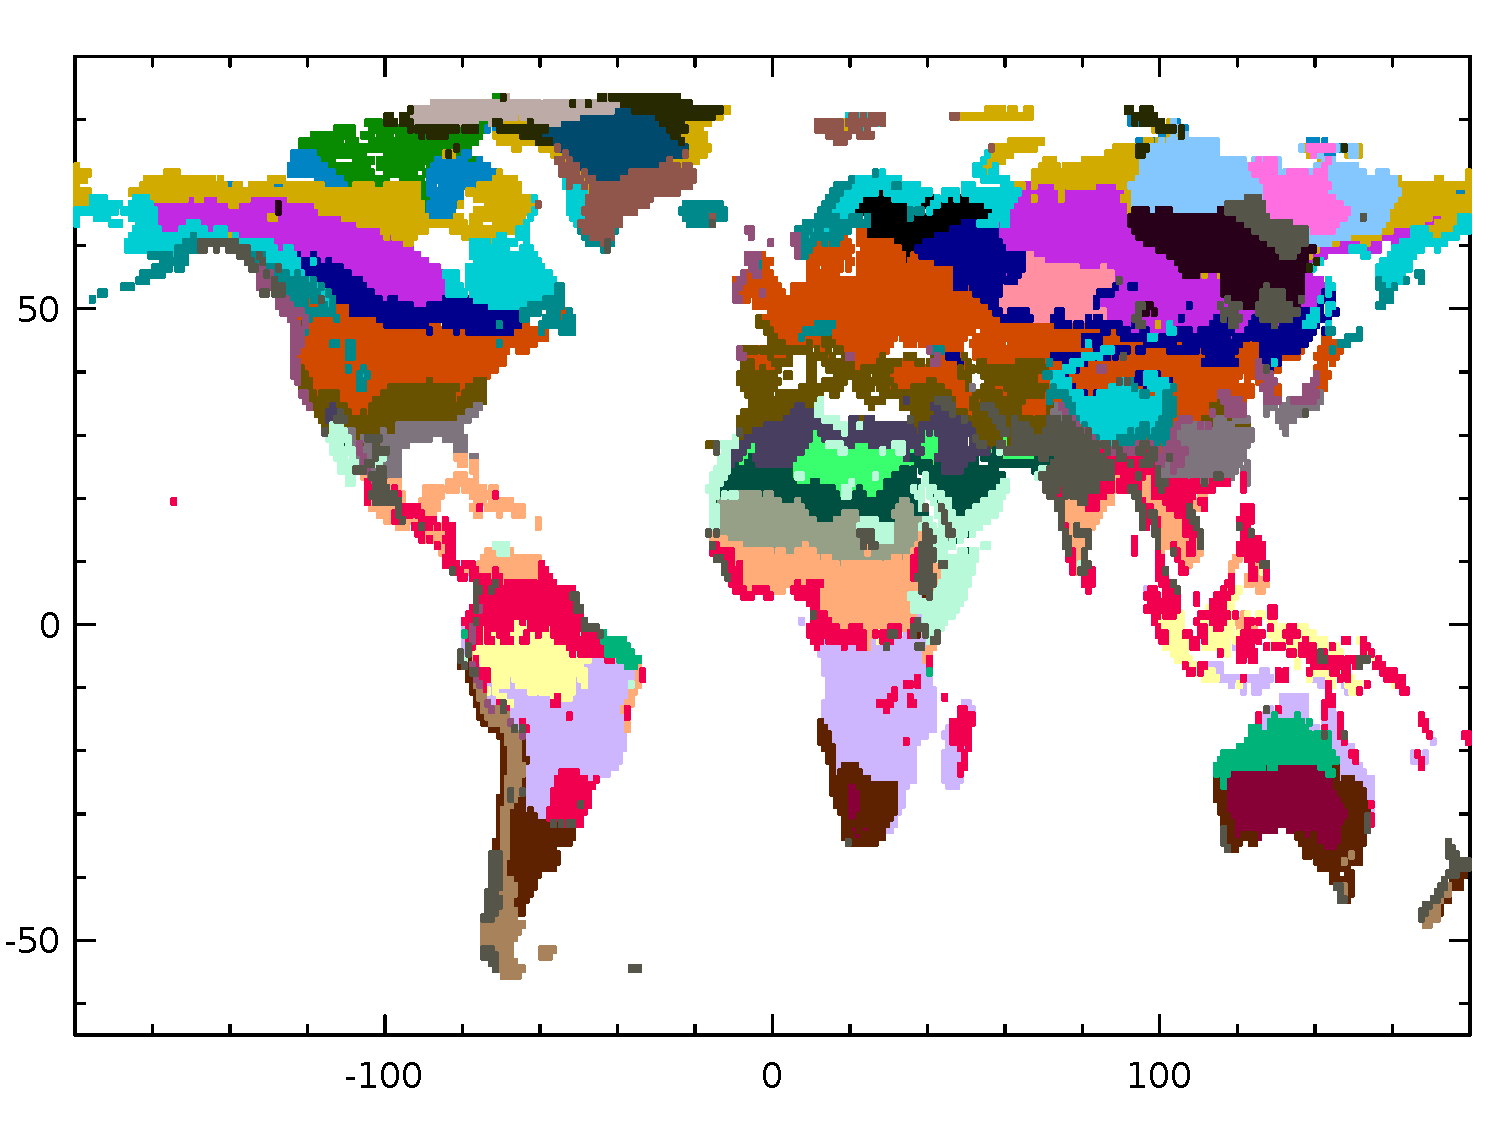
\includegraphics[width=3.5in, height=2.5in]{img/icpr-cl-lmcmdl.pdf}
    \label{fig:cl-lmcmdl}}
\hspace*{-15pt}
\subfigure[$k$-Means]{
    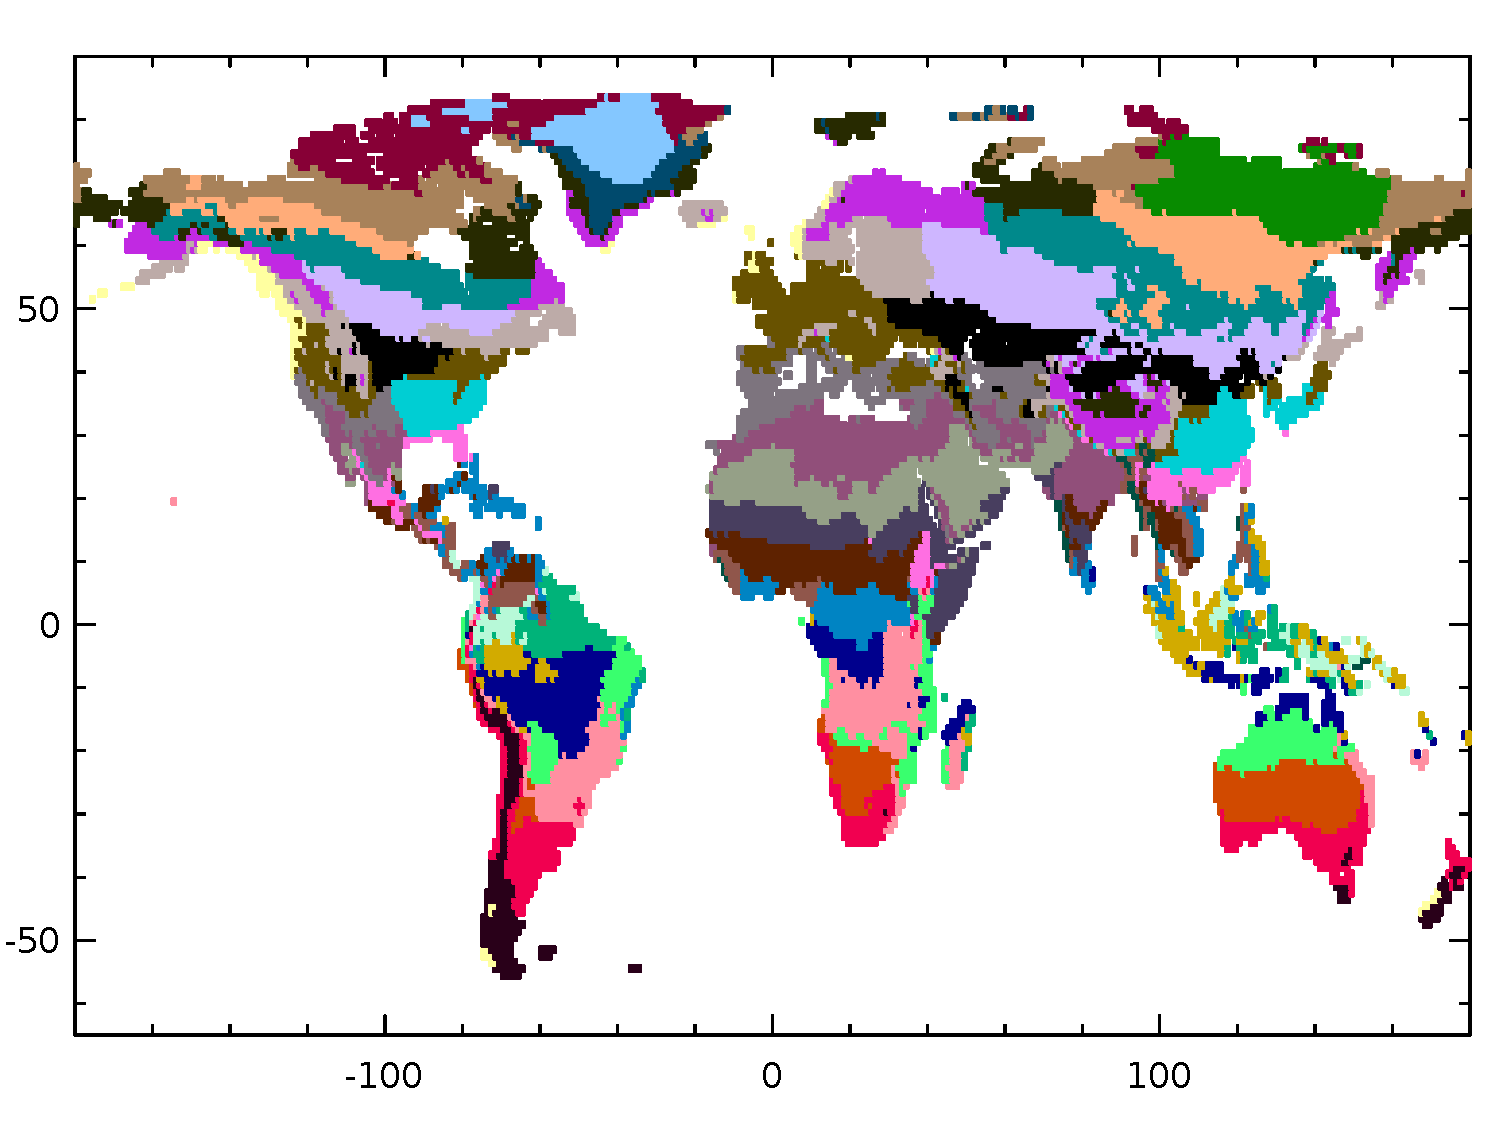
\includegraphics[width=3.5in, height=2.5in]{img/icpr-cl-kmeans.pdf}
    \label{fig:cl-kmeans}}
\hspace*{-15pt}
\subfigure[ORCLUS]{
    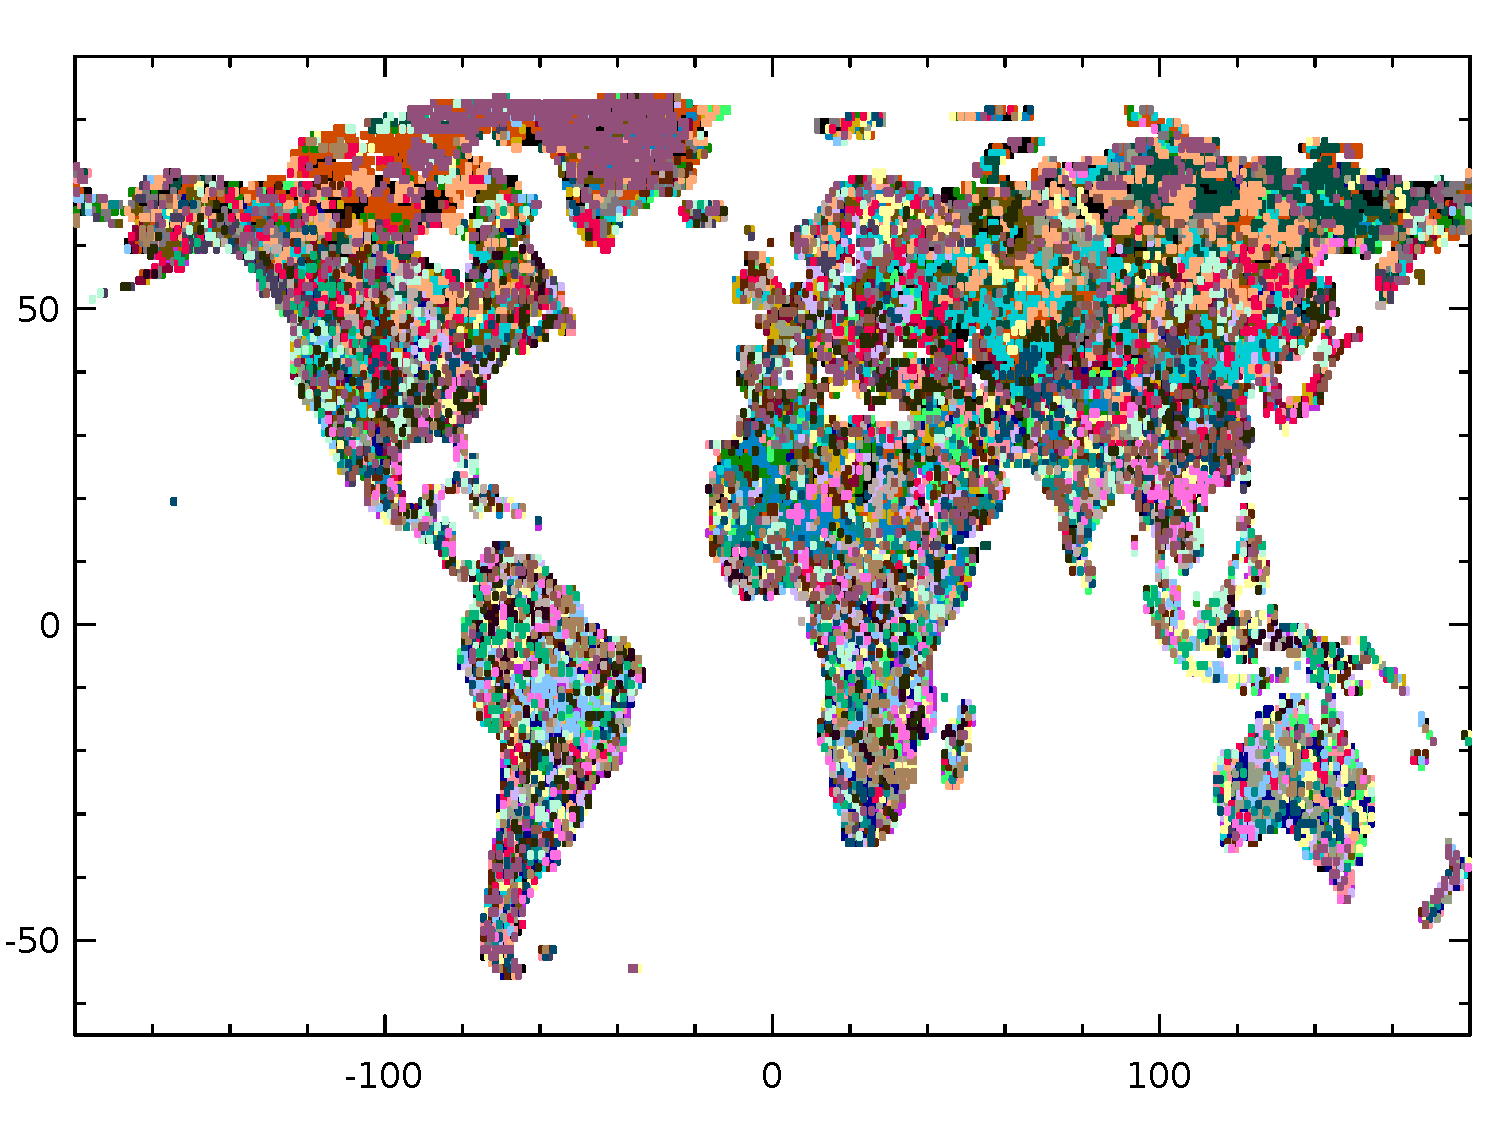
\includegraphics[width=3.5in, height=2.5in]{img/icpr-cl-orclus.pdf}
    \label{fig:cl-orclus}}
% \hspace*{-15pt}
\hspace*{0.25\textwidth}
\subfigure[K{\"o}ppen-Geiger]{
    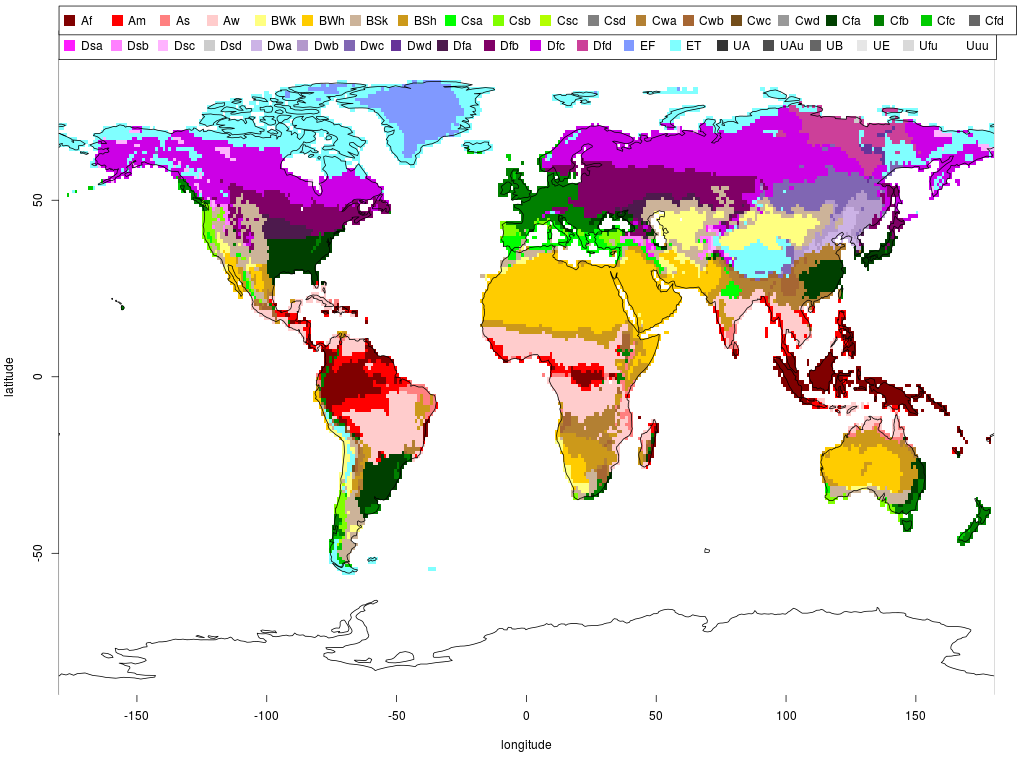
\includegraphics[width=3.5in, height=2.5in]{img/CL-KG.png}
    \label{fig:cl-kg}}
\caption{
    Results of clustering of the 24D climate dataset, composed of monthly
    averages of temperature (CRU) and precipitation (GPCC) during 1951-1980
    period, by LMCLUS \subref{fig:cl-lmclus}, by LMCLUS+MDL \subref{fig:cl-lmcmdl},
    by ORCLUS \subref{fig:cl-orclus} and $k$-Means \subref{fig:cl-kmeans}
    algorithms. For reference, K{\"o}ppen-Geiger classification is given in \subref{fig:cl-kg}.
    \emph{Note: Colors represents associations of grid cells to particular
    clusters. There is no correspondence between colors on displayed plots.}
}
\label{fig:cl-climate}
\end{figure}
}

% \IfClass{IEEEtran}{}{
% In order to compare goodness of produced clusterings we calculated the total MDL
% value of the resulting clustering for each algorithm as a sum of cluster MDL
% values. We performed the total MDL calculation with various quantization error
% values to understand how precision affects the goodness criteria.
% Figure~\ref{fig:cl-mdl} shows the effect of quantization error on the MDL value
% of clustering.
% It is clear that linear manifold clusters, which have an intrinsic
% linear structure, show better goodness-of-fit qualities reflected in
% the smaller total MDL value than the spherical zero-dimensional clusters
% produced by $k$-Means algorithm.
% %
% \begin{figure}[ht]
% \IfClass{IEEEtran}{\vspace*{-10pt}}{}
% \centering
% \includegraphics[width=3.5in]{img/cl-mdl.pdf}
% \IfClass{IEEEtran}{\vspace*{-35pt}}{}
% \caption{Total MDL value for climate dataset clustering, produced by LMCLUS and $k$-Means algorithms calculated for various user-set quantization error values.}
% \label{fig:cl-mdl}
% \end{figure}
% }
